\section{Linear Minimum Mean Square Error (LMMSE) Estimate}
\subsection{MMSE vs Linear MMSE in the Gaussian case}
\subsubsection{MMSE estimator}
\begin{itemize}
    \item The MMSE estimator of vector \(\theta\), given the observed data vector \textbf{Y}, is given by the mean vector of the \textit{a-posteriori} distribution, i.e. of the pdf of \(\theta\) conditioned to \textbf{Y}. The MSE matrix is obtained by averaging w.r.t. the data \textbf{Y} the conditional covariance matrix (the covariance matrix of the \textit{a-posteriori} pdf).
    \item When \(\theta\) and \textbf{Y} are \underline{\textbf{jointly Gaussian distributed}}, we found:
\begin{align*}
&\hat{\boldsymbol{\theta}}_{\text{MMSE}} = E\{\boldsymbol{\theta} | \mathbf{Y}\} = \boldsymbol{\eta}_{\boldsymbol{\theta}|\mathbf{Y}} = \boldsymbol{\eta}_{\boldsymbol{\theta}} + \mathbf{C}_{\boldsymbol{\theta}\mathbf{Y}}\mathbf{C}_{\mathbf{Y}}^{-1}(\mathbf{Y} - \boldsymbol{\eta}_{\mathbf{Y}}) \\[8pt]
&\text{MSE}\{\hat{\boldsymbol{\theta}}_{\text{MMSE}}\} = E\{(\boldsymbol{\theta} - \boldsymbol{\eta}_{\boldsymbol{\theta}|\mathbf{Y}})(\boldsymbol{\theta} - \boldsymbol{\eta}_{\boldsymbol{\theta}|\mathbf{Y}})^T\} = E_{\mathbf{Y}}\{\mathbf{C}_{\boldsymbol{\theta}|\mathbf{Y}}\} = \mathbf{C}_{\boldsymbol{\theta}|\mathbf{Y}} \\[8pt]
&\mathbf{C}_{\boldsymbol{\theta}|\mathbf{Y}} = E\{(\boldsymbol{\theta} - \boldsymbol{\eta}_{\boldsymbol{\theta}|\mathbf{Y}})(\boldsymbol{\theta} - \boldsymbol{\eta}_{\boldsymbol{\theta}|\mathbf{Y}})^T | \mathbf{Y}\} = \mathbf{C}_{\boldsymbol{\theta}} - \mathbf{C}_{\boldsymbol{\theta}\mathbf{Y}}\mathbf{C}_{\mathbf{Y}}^{-1}\mathbf{C}_{\mathbf{Y}\boldsymbol{\theta}}
\end{align*}
    \item In this case, the \textbf{MMSE} estimator is \underline{\textbf{linear}}, hence very easy to implent.
    \item In the case the parameter to be estimated is a \underline{scalar}, i.e. \(\theta\in\mathcal{N}(\eta_{\theta},\sigma_{\theta}^2)\), the previous equations become:
\begin{align*}
&\hat{\theta}_{\text{MMSE}} = E\{\theta | \mathbf{Y}\} = \eta_{\theta|\mathbf{Y}} = \eta_{\theta} + \mathbf{c}_{\theta\mathbf{Y}}\mathbf{C}_{\mathbf{Y}}^{-1}(\mathbf{Y} - \boldsymbol{\eta}_{\mathbf{Y}}) \\[8pt]
&\text{MSE}\{\hat{\theta}_{\text{MMSE}}\} = E\{(\theta - \eta_{\theta|\mathbf{Y}})^2\} = E_{\mathbf{Y}}\{\sigma_{\theta|\mathbf{Y}}^2\} = \sigma_{\theta|\mathbf{Y}}^2 \\[8pt]
&\sigma_{\theta|\mathbf{Y}}^2 = E\{(\theta - \eta_{\theta|\mathbf{Y}})^2 | \mathbf{Y}\} = \sigma_{\theta}^2 - \mathbf{c}_{\theta\mathbf{Y}}\mathbf{C}_{\mathbf{Y}}^{-1}\mathbf{c}_{\mathbf{Y}\theta} = \sigma_{\theta}^2 - \mathbf{c}_{\theta\mathbf{Y}}^T\mathbf{C}_{\mathbf{Y}}^{-1}\mathbf{c}_{\mathbf{Y}\theta} \\[8pt]
&\mathbf{c}_{\theta\mathbf{Y}} \triangleq E\{(\theta - \eta_{\theta})(\mathbf{Y} - \boldsymbol{\eta}_{\mathbf{Y}})^T\} = E\{(\mathbf{Y} - \boldsymbol{\eta}_{\mathbf{Y}})(\theta - \eta_{\theta})\}^T = (\mathbf{c}_{\mathbf{Y}\theta})^T \\[8pt]
&[\mathbf{c}_{\theta\mathbf{Y}}]_{i} = E\{(\theta - \eta_{\theta})(Y_{i} - \eta_{Y_i})\}, \quad i=0, 1, 2, \dots, N-1
\end{align*}
    \item In the case also the data vector \textbf{Y} is a \underline{scalar}, i.e. \(N=1\) and \textbf{Y}=Y, we found the well-known "\textbf{\underline{regression line}}":
    \begin{align*}
\hat{\theta}_{\text{MMSE}} &= E\{\theta | Y\} = \eta_{\theta|Y} = \eta_{\theta} + c_{\theta Y} (\sigma_{Y}^2)^{-1} (Y - \eta_{Y}) \\[8pt]
&= \eta_{\theta} + \rho_{\theta Y} \sigma_{\theta} \sigma_{Y} (\sigma_{Y}^2)^{-1} (Y - \eta_{Y}) \\[8pt]
&= \eta_{\theta} + \rho_{\theta Y} \frac{\sigma_{\theta}}{\sigma_{Y}} (Y - \eta_{Y}) \\[8pt]
\text{MSE}\{\hat{\theta}_{\text{MMSE}}\} &= E\{(\theta - \eta_{\theta|Y})^2\} = E_{Y} \{\sigma_{\theta|Y}^2\} = \sigma_{\theta|Y}^2 \\[6pt]
\sigma_{\theta|Y}^2 &= E\{(\theta - \eta_{\theta|Y})^2 | Y\} = \sigma_{\theta}^2 - c_{\theta Y} (\sigma_{Y}^2)^{-1} c_{\theta Y} = \sigma_{\theta}^2 - \frac{(\rho_{\theta Y} \sigma_{\theta} \sigma_{Y})^2}{\sigma_{Y}^2} \\[6pt]
&= \sigma_{\theta}^2 (1 - \rho_{\theta Y}^2)
\end{align*}
\end{itemize}
\subsubsection{Linear MMSE estimator: the scalar case}
\begin{itemize}
\item If the parameter vector \(\theta\) to be estimated and the observed data \textbf{Y} are \underline{\textbf{not}} \textbf{jointly Gaussian}, the derivation of the mean (or even of the mode) of the \textit{a-posteriori} pdf can be very cumbersome and sometimes unfeasible, at least in closed form.
\item The MMSE/MAP estimators are in general \textbf{non-linear}, so they may be difficult to implement. Sometimes the implementation requires numerical calculations to converge to the optimal solution.
\item If it is of fundamental importance to keep \textbf{low} the \textbf{computational complexity}, a possibile approach is to impose the estimator to be \textbf{linear} and to look for the coefficients of the linear combination that minimize the MSE:
\[
\rightarrow \textbf{Linear Minimum Mean Square Error (LMMSE)}
\]

\item Let us derive first the \textbf{LMMSE} in the simple case of scalar parameter \(\theta\) to be estimated and scalar observed data \(Y\):
\begin{align*}
\hat{\theta}&=aY+b \quad \rightarrow \quad \varepsilon=\theta-\hat{\theta}=\theta-aY-b
\end{align*}

\item The \textbf{LMMSE} estimator is obtained by looking for the values of parameters \(a\) and \(b\) that minimize the MSE:

\begin{align*}
\varepsilon &= \theta - \hat{\theta} = \theta - aY - b \quad \rightarrow \quad \text{MSE}\{\hat{\theta}\} = E\{\varepsilon^2\} = E\{(\theta - aY - b)^2\}
\end{align*}
\item The optimal solution can be found by differentiating the MSE w.r.t. \(a\) e \(b\), setting the derivatives equal to 0 and solving the system of two linear equations in the two unknowns:
\[
\begin{cases}
    \frac{\partial E\{\varepsilon^2\}}{\partial b}=0\\[8pt]
    \frac{\partial E\{\varepsilon ^2\}}{\partial a} =0
\end{cases}
\]
\begin{align*}
\text{MSE}\{\hat{\theta}\} &= E\{\varepsilon^2\} = E\{(\theta - aY - b)^2\} \\[8pt]
\frac{\partial E\{\varepsilon^2\}}{\partial b} &= \frac{\partial E\{(\theta - aY - b)^2\}}{\partial b} = E\left\{\frac{\partial\{(\theta - aY - b)^2\}}{\partial b}\right\} = -2E\{(\theta - aY - b)\} \\[8pt]
&= -2E\{\varepsilon\} = 0 \quad \rightarrow \quad \text{unbiased estimator} \\[8pt]
\frac{\partial E\{\varepsilon^2\}}{\partial a} &= \frac{\partial E\{(\theta - aY - b)^2\}}{\partial a} = E\left\{\frac{\partial\{(\theta - aY - b)^2\}}{\partial a}\right\} = E\{-2Y (\theta - aY - b)\} \\[8pt]
&= -2E\{Y\varepsilon\} = 0 \quad \rightarrow \quad \text{error} \perp \text{data (Ortogonality Principle)}
\end{align*}

\item \textbf{The LMMSE estimator is derived by imposing that the estimator is unbiased and the estimation error is orthogonal to the observed data}
\item Let us derive explicitly the values of the parameters \(a\) and \(b\) which minimize the MSE.
\item From the \(1^{st}\) equation we get \(b\):
\begin{align*}
E\{\theta - aY - b\} = 0 \quad \rightarrow \quad \eta_{\theta} - a\eta_{Y} - b = 0 \quad \rightarrow \quad b = \eta_{\theta} - a\eta_{Y}
\end{align*}
\item Then, we insert \(b\) in the \(2^{nd}\) equation and we solve w.r.t. \(a\):
\begin{align*}
&E\{Y\varepsilon\} = E\{Y(\theta - aY - b)\} = E\{Y(\theta - aY - (\eta_{\theta} - a\eta_{Y}))\} = 0 \\[8pt]
&E\{Y(\theta - \eta_{\theta} - a(Y - \eta_{Y}))\} = 0 \\[8pt]
&E\{Y(\theta - \eta_{\theta} - a(Y - \eta_{Y}))\} - \underbrace{E\{\eta_{Y}(\theta - \eta_{\theta} - a(Y - \eta_{Y}))\}}_{=E\{\eta_{Y} \varepsilon\} = \eta_{Y} E\{\varepsilon\}=0} = 0 \\[8pt]
&E\{(Y - \eta_{Y})(\theta - \eta_{\theta} - a(Y - \eta_{Y}))\}=0 \\[8pt]
&E\{(Y - \eta_{Y})(\theta - \eta_{\theta} - a(Y - \eta_{Y}))\} = c_{Y\theta} - a\sigma_{Y}^2 = 0
\end{align*}
\item We can derive:
\begin{align*}
a &= \frac{c_{Y\theta}}{\sigma_{Y}^2} = \frac{\rho_{Y\theta}\sigma_{\theta}\sigma_{Y}}{\sigma_{Y}^2} = \rho_{Y\theta}\frac{\sigma_{\theta}}{\sigma_{Y}} \quad \rightarrow \quad b = \eta_{\theta} - a\eta_{Y} = \eta_{\theta} - \rho_{Y\theta}\frac{\sigma_{\theta}}{\sigma_{Y}}\eta_{Y} \\[8pt]
&\hat{\theta}_{\text{LMMSE}} = \rho_{Y\theta}\frac{\sigma_{\theta}}{\sigma_{Y}}Y + \eta_{\theta} - \rho_{Y\theta}\frac{\sigma_{\theta}}{\sigma_{Y}}\eta_{Y} = \eta_{\theta} + \rho_{Y\theta}\frac{\sigma_{\theta}}{\sigma_{Y}}(Y - \eta_{Y})
\end{align*}

\item It is worth observing that \underline{the LMMSE estimator coincides with the MMSE estimator in the Gaussian case}. Hence, this linear estimator is the optimal MMSE estimator when the parameter to be estimated and the data are jointly Gaussian and it is the best linear unbiased estimator in all the other (non-Gaussian) cases.
\begin{align*}
\text{MSE}\{\hat{\theta}_{\text{LMMSE}}\} &= E\{\varepsilon^2\} = E\{(\theta - aY - b)\varepsilon\} = E\{\theta\varepsilon\} - aE\{Y\varepsilon\} - bE\{\varepsilon\} \\[8pt]
&= E\{\theta\varepsilon\} = E\{\theta\varepsilon\} - \eta_{\theta}E\{\varepsilon\} = E\{(\theta - \eta_{\theta})\varepsilon\} \\[8pt]
&= E\left\{(\theta - \eta_{\theta})\left(\theta - \eta_{\theta} - \rho_{\theta Y}\frac{\sigma_{\theta}}{\sigma_{Y}}(Y - \eta_{Y})\right)\right\} \\[8pt]
&= E\{(\theta - \eta_{\theta})^2\} - \rho_{\theta Y}\frac{\sigma_{\theta}}{\sigma_{Y}}E\{(\theta - \eta_{\theta})(Y - \eta_{Y})\} \\[8pt]
&= \sigma_{\theta}^2 - \rho_{\theta Y}\frac{\sigma_{\theta}}{\sigma_{Y}}(\rho_{\theta Y}\sigma_{\theta}\sigma_{Y}) \\[8pt]
&= \sigma_{\theta}^2(1 - \rho_{\theta Y}^2)
\end{align*}
\item The MSE of the LMMSE estimator obviously coincides with that of the MMSE estimator in the Gaussian case: it is a function of the variance of the parameter \(\theta\) to be estimated and of the correlation coefficient between \(\theta\) and the data \(Y\).
\item \underline{\textbf{Geometrical interpretation}}: Assume a linear vector space where the element of the space are random variables and where the \textbf{scalar product} and the \textbf{norm} are defined as follows:
\begin{align*}
&(Y, \theta) \triangleq \text{cov}\{Y, \theta\} = E\{(Y - \eta_{Y})(\theta - \eta_{\theta})\} = c_{Y\theta} \\[8pt]
&\|Y\| \triangleq \sqrt{(Y, Y)} = \sqrt{E\{(Y - \eta_{Y})^2\}} = \sqrt{\text{var}\{Y\}} = \sigma_{Y} \\[8pt]
&(Y, \theta) = 0 \quad \Rightarrow \quad Y \perp \theta
\end{align*}
\item Let us define now the unit-norm element of the space that is collinear with \(Y\):

\begin{align*}
I_{Y} &\triangleq \frac{Y - \eta_{Y}}{\sigma_{Y}} = \frac{Y - \eta_{Y}}{\|Y\|} \quad \Rightarrow \quad \|I_{Y}\|=1
\end{align*}
\begin{figure}[H]
    \centering
    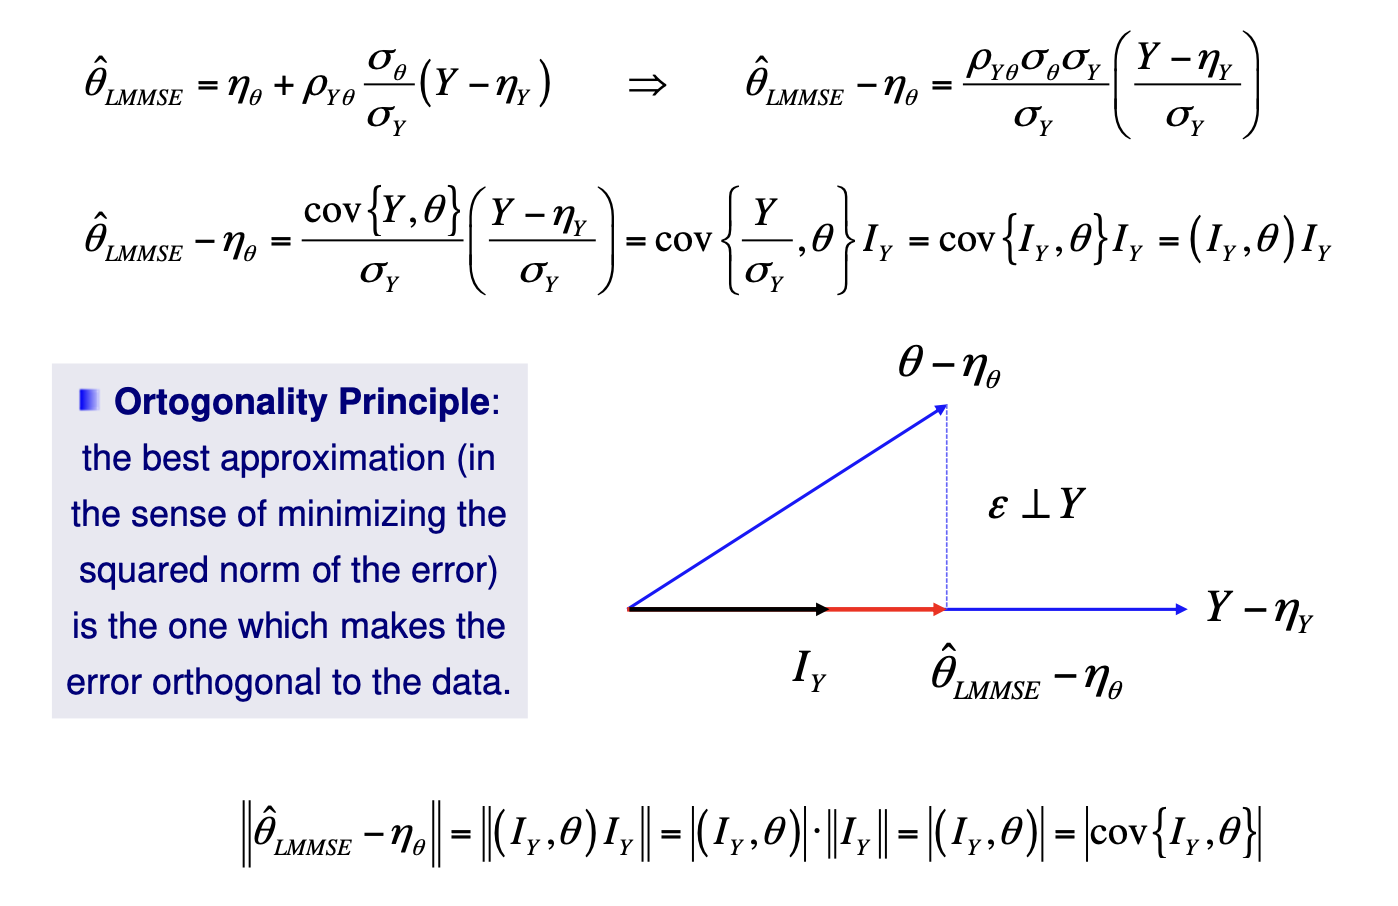
\includegraphics[width=0.55\linewidth]{Image/pdf 8/1.Orthogonality_principle.png}
    \label{fig:placeholder}
\end{figure}
\begin{figure}[H]
    \centering
    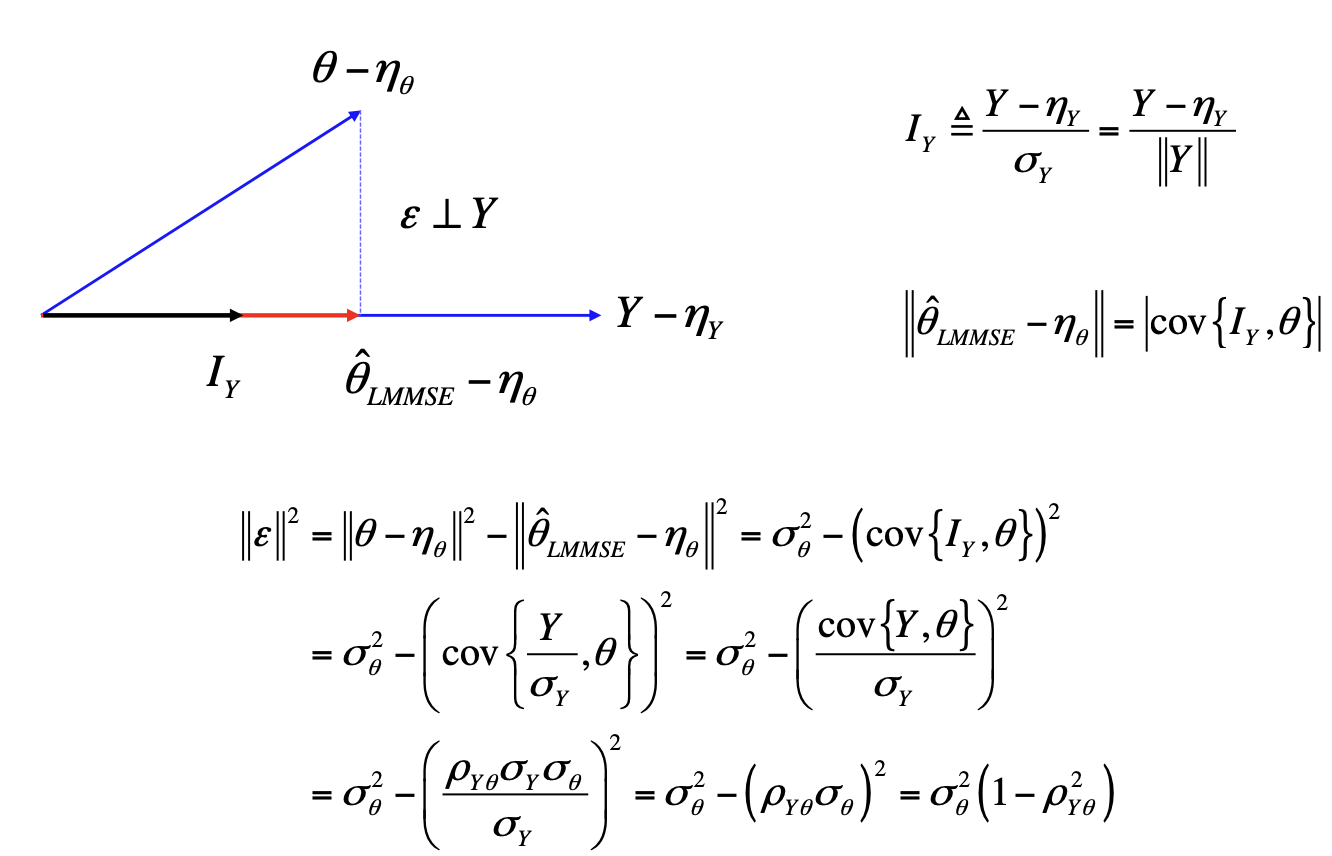
\includegraphics[width=0.55\linewidth]{Image/pdf 8/2.Orthogonality_2.png}
    \label{fig:placeholder}
\end{figure}
(ESERCIZIO DA SLIDE 8, 14-22)
\end{itemize}
\subsection{LMMSE estimator: multiple observations}
\begin{itemize}
    \item Let us now derive the \textbf{LMMSE} estimator of the parameter \(\theta\) in the case of multiple observed data: \textbf{Y} is an \(N-\)dimensional vector.
    \begin{align*}
&\hat{\theta} = \sum_{i=1}^{N} a_{i}Y_{i} + b = \mathbf{a}^{T}\mathbf{Y} + b, \quad \varepsilon = \theta - \hat{\theta} = \theta - \mathbf{a}^{T}\mathbf{Y} - b \\[8pt]
&\text{MSE}\{\hat{\theta}\} = E\{\varepsilon^2\} = E\{(\theta - \mathbf{a}^{T}\mathbf{Y} - b)^2\} \\[8pt]
&\frac{\partial E\{\varepsilon^2\}}{\partial b} = \frac{\partial E\{(\theta - \mathbf{a}^{T}\mathbf{Y} - b)^2\}}{\partial b} = E\left\{\frac{\partial\{(\theta - \mathbf{a}^{T}\mathbf{Y} - b)^2\}}{\partial b}\right\} = -2E\{(\theta - \mathbf{a}^{T}\mathbf{Y} - b)\} \\[8pt]
&= -2E\{\varepsilon\} = 0 \quad \rightarrow \quad \text{unbiased estimator} \\[8pt]
&E\{\varepsilon\}=0 \rightarrow \quad E\{\theta - \mathbf{a}^{T}\mathbf{Y} - b\} = \eta_{\theta} - \mathbf{a}^{T}\boldsymbol{\eta}_{\mathbf{Y}} - b = 0 \quad \rightarrow \quad b = \eta_{\theta} - \mathbf{a}^{T}\boldsymbol{\eta}_{\mathbf{Y}}
\end{align*}
\item Let us now insert \(b\) in the expression of the MSE and minimize the result w.r.t. vector \textbf{a}:
\begin{align*}
\text{MSE}\{\hat{\theta}\} &= E\{\varepsilon^2\} = E\{(\theta - \mathbf{a}^{T}\mathbf{Y} - b)^2\} \\[8pt]
&= E\{(\theta - \mathbf{a}^{T}\mathbf{Y} - \eta_{\theta} + \mathbf{a}^{T}\boldsymbol{\eta}_{\mathbf{Y}})^2\} \\[8pt]
&= E\{(\theta - \eta_{\theta} - \mathbf{a}^{T}(\mathbf{Y} - \boldsymbol{\eta}_{\mathbf{Y}}))^2\} \\[8pt]
&= E\{(\theta - \eta_{\theta} - \mathbf{a}^{T}(\mathbf{Y} - \boldsymbol{\eta}_{\mathbf{Y}}))(\theta - \eta_{\theta} - \mathbf{a}^{T}(\mathbf{Y} - \boldsymbol{\eta}_{\mathbf{Y}}))^T\} \\[8pt]
&= E\{(\theta - \eta_{\theta})^2\} - \mathbf{a}^{T}E\{(\mathbf{Y} - \boldsymbol{\eta}_{\mathbf{Y}})(\theta - \eta_{\theta})\} - E\{(\theta - \eta_{\theta})(\mathbf{Y} - \boldsymbol{\eta}_{\mathbf{Y}})^{T}\}\mathbf{a} \\[8pt]
&\quad +\mathbf{a}^{T}E\{(\mathbf{Y} - \boldsymbol{\eta}_{\mathbf{Y}})(\mathbf{Y} - \boldsymbol{\eta}_{\mathbf{Y}})^{T}\}\mathbf{a} \\[8pt]
&= \sigma_{\theta}^2 - \mathbf{a}^{T}\mathbf{c}_{\mathbf{Y}\theta} - \mathbf{c}_{\theta\mathbf{Y}}\mathbf{a} + \mathbf{a}^{T}\mathbf{C}_{\mathbf{Y}}\mathbf{a} \\[8pt]
&= \sigma_{\theta}^2 - 2\mathbf{a}^{T}\mathbf{c}_{\mathbf{Y}\theta} + \mathbf{a}^{T}\mathbf{C}_{\mathbf{Y}}\mathbf{a}
\end{align*}
\item The optimal vector \(a\) is derived by calculating the gradient of the MSE w.r.t. \textbf{a}, setting the gradient equal to 0, and solving the equation w.r.t. \textbf{a}:
\begin{align*}
\nabla_{\mathbf{a}}\text{MSE}\{\hat{\theta}\} &= \nabla_{\mathbf{a}}(\sigma_{\theta}^2 - 2\mathbf{a}^{T}\mathbf{c}_{\mathbf{Y}\theta} + \mathbf{a}^{T}\mathbf{C}_{\mathbf{Y}}\mathbf{a}) = -2\mathbf{c}_{\mathbf{Y}\theta} + 2\mathbf{C}_{\mathbf{Y}}\mathbf{a} = 0 \\[8pt]
\mathbf{a} &= \mathbf{C}_{\mathbf{Y}}^{-1}\mathbf{c}_{\mathbf{Y}\theta} \quad \rightarrow \quad b = \eta_{\theta} - \mathbf{c}_{\theta\mathbf{Y}}\mathbf{C}_{\mathbf{Y}}^{-1}\boldsymbol{\eta}_{\mathbf{Y}} \\[8pt]
\hat{\theta}_{\text{LMMSE}} &= \mathbf{c}_{\theta\mathbf{Y}}\mathbf{C}_{\mathbf{Y}}^{-1}\mathbf{Y} + \eta_{\theta} - \mathbf{c}_{\theta\mathbf{Y}}\mathbf{C}_{\mathbf{Y}}^{-1}\boldsymbol{\eta}_{\mathbf{Y}} = \eta_{\theta} + \mathbf{c}_{\theta\mathbf{Y}}\mathbf{C}_{\mathbf{Y}}^{-1}(\mathbf{Y} - \boldsymbol{\eta}_{\mathbf{Y}})
\end{align*}
\item Which, again, coincides with the MMSE estimator for the Gaussian case.
\item The MSE of the LMMSE estimator can be obtained by inserting the optimal \textbf{a} in the MSE formula previously derived:
\begin{align*}
\text{MSE}\{\hat{\theta}_{\text{LMMSE}}\} &= \left[\sigma_{\theta}^2 - 2\mathbf{a}^{T}\mathbf{c}_{\mathbf{Y}\theta} + \mathbf{a}^{T}\mathbf{C}_{\mathbf{Y}}\mathbf{a}\right]_{\mathbf{a}=\mathbf{C}_{\mathbf{Y}}^{-1}\mathbf{c}_{\mathbf{Y}\theta}} \\[8pt]
&= \sigma_{\theta}^2 - 2\left(\mathbf{C}_{\mathbf{Y}}^{-1}\mathbf{c}_{\mathbf{Y}\theta}\right)^{T}\mathbf{c}_{\mathbf{Y}\theta} + \left(\mathbf{C}_{\mathbf{Y}}^{-1}\mathbf{c}_{\mathbf{Y}\theta}\right)^{T}\mathbf{C}_{\mathbf{Y}}\mathbf{C}_{\mathbf{Y}}^{-1}\mathbf{c}_{\mathbf{Y}\theta} \\[8pt]
&= \sigma_{\theta}^2 - 2\mathbf{c}_{\mathbf{Y}\theta}^{T}\left(\mathbf{C}_{\mathbf{Y}}^{-1}\right)^{T}\mathbf{c}_{\mathbf{Y}\theta} + \mathbf{c}_{\mathbf{Y}\theta}^{T}\left(\mathbf{C}_{\mathbf{Y}}^{-1}\right)^{T}\mathbf{C}_{\mathbf{Y}}\mathbf{C}_{\mathbf{Y}}^{-1}\mathbf{c}_{\mathbf{Y}\theta} \\[8pt]
&= \sigma_{\theta}^2 - 2\mathbf{c}_{\theta\mathbf{Y}}\mathbf{C}_{\mathbf{Y}}^{-1}\mathbf{c}_{\mathbf{Y}\theta} + \mathbf{c}_{\theta\mathbf{Y}}\mathbf{C}_{\mathbf{Y}}^{-1}\mathbf{C}_{\mathbf{Y}}\mathbf{C}_{\mathbf{Y}}^{-1}\mathbf{c}_{\mathbf{Y}\theta} \\[8pt]
&= \sigma_{\theta}^2 - \mathbf{c}_{\theta\mathbf{Y}}\mathbf{C}_{\mathbf{Y}}^{-1}\mathbf{c}_{\mathbf{Y}\theta}
\end{align*}
$$
\boxed{
\text{MSE}\{\hat{\theta}_{\text{LMMSE}}\} = \sigma_{\theta}^2 - \mathbf{c}_{\theta\mathbf{Y}}\mathbf{C}_{\mathbf{Y}}^{-1}\mathbf{c}_{\mathbf{Y}\theta}}
$$
\item In summary, \underline{the parameter \(b\) is chosen in suca a way that the LMMSE estimator is \textbf{unbiased}}:
\begin{align*}
E\{\theta - \hat{\theta}_{\text{LMMSE}}\} &= E\{\theta\} - E\left\{\eta_{\theta} + \mathbf{c}_{\theta\mathbf{Y}}\mathbf{C}_{\mathbf{Y}}^{-1}(\mathbf{Y} - \boldsymbol{\eta}_{\mathbf{Y}})\right\} \\[8pt]
&= \eta_{\theta} - \left(E\{\eta_{\theta}\} + \mathbf{c}_{\theta\mathbf{Y}}\mathbf{C}_{\mathbf{Y}}^{-1}E\{\mathbf{Y} - \boldsymbol{\eta}_{\mathbf{Y}}\}\right) \\[8pt]
&= \eta_{\theta} - (\eta_{\theta} + \mathbf{c}_{\theta\mathbf{Y}}\mathbf{C}_{\mathbf{Y}}^{-1}\mathbf{0}) \\[8pt]
&= \eta_{\theta} - \eta_{\theta} = 0
\end{align*}
\item \underline{The vector \textbf{a} is chosen in such a way that the estimation errori is orthogonal to the data}\\ \noindent \underline{ (\textbf{Orthogonality principle})}:\(E\{\varepsilon Y_i\}=0,\quad i=1,2,\cdots, N\)
\begin{align*}
E\{\varepsilon\mathbf{Y}^{T}\} &= E\{\varepsilon\mathbf{Y}^{T}\} - E\{\varepsilon\}\boldsymbol{\eta}_{\mathbf{Y}}^{T} = E\{\varepsilon(\mathbf{Y} - \boldsymbol{\eta}_{\mathbf{Y}})^{T}\} \\[8pt]
&= E\left\{\left(\theta - \eta_{\theta} - \mathbf{a}^{T}(\mathbf{Y} - \boldsymbol{\eta}_{\mathbf{Y}})\right)(\mathbf{Y} - \boldsymbol{\eta}_{\mathbf{Y}})^{T}\right\} \\[8pt]
&= \mathbf{c}_{\theta\mathbf{Y}} - \mathbf{a}^{T}\mathbf{C}_{\mathbf{Y}} = \mathbf{c}_{\theta\mathbf{Y}} - \mathbf{c}_{\theta\mathbf{Y}}\mathbf{C}_{\mathbf{Y}}^{-1}\mathbf{C}_{\mathbf{Y}} = \mathbf{c}_{\theta\mathbf{Y}} - \mathbf{c}_{\theta\mathbf{Y}} = \mathbf{0}
\end{align*}
\vspace{-0.5em}
$$
\text{since } \mathbf{c}_{\theta\mathbf{Y}} = (\mathbf{c}_{\mathbf{Y}\theta})^{T}
$$
\item Also say:
\begin{align*}
\hat{\theta}_{\text{LMMSE}} &= \eta_{\theta} + \mathbf{c}_{\theta\mathbf{Y}}\mathbf{C}_{\mathbf{Y}}^{-1}(\mathbf{Y} - \boldsymbol{\eta}_{\mathbf{Y}}) \quad \implies \quad \hat{\theta}_{\text{LMMSE}} - \eta_{\theta} = \mathbf{c}_{\theta\mathbf{Y}}\mathbf{C}_{\mathbf{Y}}^{-1/2}\mathbf{C}_{\mathbf{Y}}^{-1/2}(\mathbf{Y} - \boldsymbol{\eta}_{\mathbf{Y}}) \\[8pt]
\mathbf{I}_{\mathbf{Y}} &\triangleq \mathbf{C}_{\mathbf{Y}}^{-1/2}(\mathbf{Y} - \boldsymbol{\eta}_{\mathbf{Y}}) \quad \text{data whitening (decorrelation)} \\[8pt]
\boldsymbol{\eta}_{\mathbf{I}_{\mathbf{Y}}} &= E\{\mathbf{I}_{\mathbf{Y}}\} = E\left\{\mathbf{C}_{\mathbf{Y}}^{-1/2}(\mathbf{Y} - \boldsymbol{\eta}_{\mathbf{Y}})\right\} = \mathbf{C}_{\mathbf{Y}}^{-1/2}E\{\mathbf{Y} - \boldsymbol{\eta}_{\mathbf{Y}}\} = \mathbf{0} \\[8pt]
\mathbf{C}_{\mathbf{I}_{\mathbf{Y}}} &= E\{\mathbf{I}_{\mathbf{Y}}\mathbf{I}_{\mathbf{Y}}^{T}\} = E\left\{\mathbf{C}_{\mathbf{Y}}^{-1/2}(\mathbf{Y} - \boldsymbol{\eta}_{\mathbf{Y}})(\mathbf{Y} - \boldsymbol{\eta}_{\mathbf{Y}})^{T}\mathbf{C}_{\mathbf{Y}}^{-1/2}\right\} \\[8pt]
&= \mathbf{C}_{\mathbf{Y}}^{-1/2}E\left\{(\mathbf{Y} - \boldsymbol{\eta}_{\mathbf{Y}})(\mathbf{Y} - \boldsymbol{\eta}_{\mathbf{Y}})^{T}\right\}\mathbf{C}_{\mathbf{Y}}^{-1/2} \\[8pt]
&= \mathbf{C}_{\mathbf{Y}}^{-1/2}\mathbf{C}_{\mathbf{Y}}\mathbf{C}_{\mathbf{Y}}^{-1/2} = \mathbf{C}_{\mathbf{Y}}^{-1/2}\mathbf{C}_{\mathbf{Y}}^{1/2}\mathbf{C}_{\mathbf{Y}}^{1/2}\mathbf{C}_{\mathbf{Y}}^{-1/2} \\[8pt]
&= \mathbf{I} \quad [N \times N \text{ identity matrix}]
\end{align*}
\item hence, the elements of vector \(\mathbf{I}_Y\) are zero mean random variables, mutually uncorrelated and with unit variance.
\begin{figure}
    \centering
    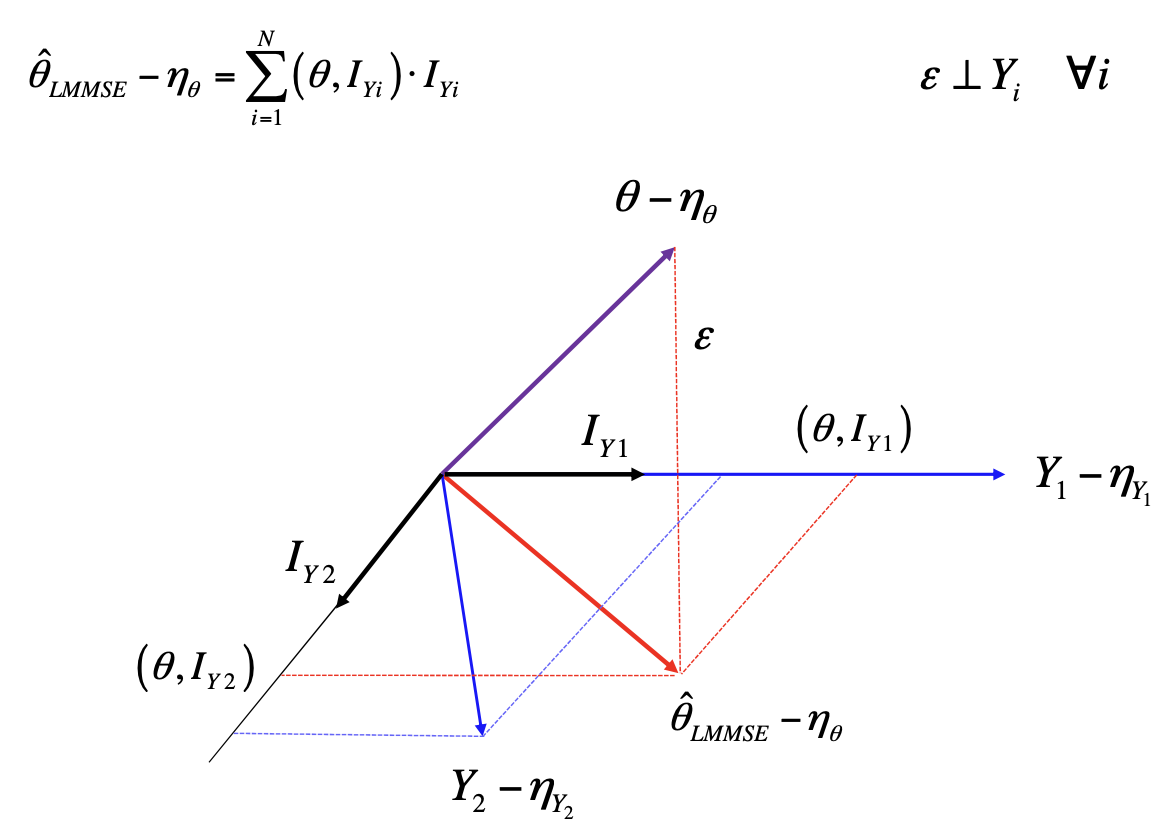
\includegraphics[width=0.55\linewidth]{Image/pdf 8/3.Geom.png}
    \label{fig:placeholder}
\end{figure}
(ESERCIZI DA 8, 31-81)
\end{itemize}
\subsection{Vector LMMSE estimator}
\begin{itemize}
\item The \textbf{LMMSE estimator} of the random vector \(\theta\) is a simple generalization of the scalar one, and obviously coincides with the MMSE estimator Gaussian case:
\[
\begin{cases}
\hat{\theta}_{\text{LMMSE}} = \eta_{\theta} + \mathbf{c}_{\theta\mathbf{Y}}\mathbf{C}_{\mathbf{Y}}^{-1}(\mathbf{Y} - \boldsymbol{\eta}_{\mathbf{Y}}) \\[8pt]
\text{MSE}\{\hat{\theta}_{\text{LMMSE}}\} = \mathbf{C}_{\theta} - \mathbf{c}_{\theta\mathbf{Y}}\mathbf{C}_{\mathbf{Y}}^{-1}\mathbf{c}_{\mathbf{Y}\theta}
\end{cases}
\]
\item It is important to stress that to implement the \textbf{LMMSE estimator} of \(\theta\) \underline{it is not necessary to know}\\ \noindent \underline{the joint pdf of \(\theta\) and \textbf{Y}}, but we need only to know some 1st and 2nd order statistics.
\item Mean vector and covariance matrix of the vector \(\theta\) we want to estimate:
\[
\begin{cases}
\boldsymbol{\eta}_{\boldsymbol{\theta}} &= E\{\boldsymbol{\theta}\} \\[8pt]
\mathbf{C}_{\boldsymbol{\theta}} &= E\{(\boldsymbol{\theta} - \boldsymbol{\eta}_{\boldsymbol{\theta}})(\boldsymbol{\theta} - \boldsymbol{\eta}_{\boldsymbol{\theta}})^{T}\} \quad (p \times p \text{ matrix})
\end{cases}
\]
\item Cross-covariance matrix between the data vector \textbf{Y} and the vector \(\theta\) we want to estimate:
$$
\mathbf{C}_{\mathbf{Y}\boldsymbol{\theta}} = E\left\{(\mathbf{Y} - \boldsymbol{\eta}_{\mathbf{Y}})(\boldsymbol{\theta} - \boldsymbol{\eta}_{\boldsymbol{\theta}})^{T}\right\}
\quad (N \times p \text{ matrix})
$$

\item Mean vector and covariance matrix of the data vector \(\textbf{Y}\rightarrow\mathbf{C}_Y\) is necessary for the data \textit{whitening}.
\[
\begin{cases}
\boldsymbol{\eta}_{\mathbf{Y}} &= E\{\mathbf{Y}\} \\[8pt]
\mathbf{C}_{\mathbf{Y}} &= E\{(\mathbf{Y} - \boldsymbol{\eta}_{\mathbf{Y}})(\mathbf{Y} - \boldsymbol{\eta}_{\mathbf{Y}})^{T}\} \quad (N \times N \text{ matrix})
\end{cases}
\]
\end{itemize}
\subsubsection{LMMSE estimator for the Bayesian Linear Model}
\begin{itemize}
    \item The \textbf{LMMSE} estimator in the case the observed data are represented by the \underline{\textbf{Bayesian Linear Model}}, i.e. \(\theta\) is random, but not necessarily Gaussian distributed, embedded in additive noise (AWN), not necessarily Guassian distributed:
    \begin{figure}[H]
        \centering
        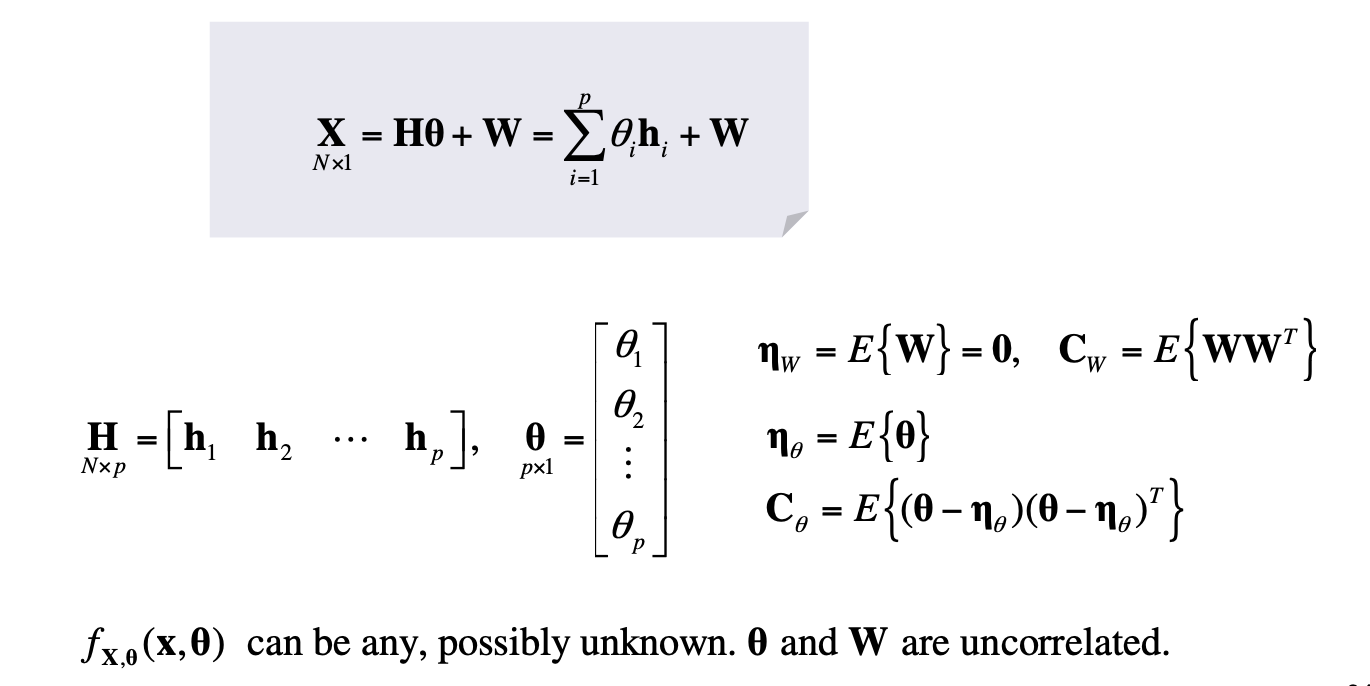
\includegraphics[width=0.75\linewidth]{Image/pdf 8/4.Formula.png}
        \label{fig:placeholder}
    \end{figure}
\vspace{-1.5em}
\begin{align*}
&\boldsymbol{\eta}_{\mathbf{X}} = E\{\mathbf{X}\} = \mathbf{H}\boldsymbol{\eta}_{\boldsymbol{\theta}} \\[8pt]
&\mathbf{C}_{\mathbf{X}} = E\{(\mathbf{X} - \boldsymbol{\eta}_{\mathbf{X}})(\mathbf{X} - \boldsymbol{\eta}_{\mathbf{X}})^{T}\} = \mathbf{H}\mathbf{C}_{\boldsymbol{\theta}}\mathbf{H}^{T} + \mathbf{C}_{\mathbf{W}} \\[8pt]
&\mathbf{C}_{\mathbf{X}\boldsymbol{\theta}} = E\{(\mathbf{X} - \boldsymbol{\eta}_{\mathbf{X}})(\boldsymbol{\theta} - \boldsymbol{\eta}_{\boldsymbol{\theta}})^{T}\} = \mathbf{H}\mathbf{C}_{\boldsymbol{\theta}}
\end{align*}
\item Inserting these relations in the general expressions of the LMMSE estimator, we get the \textbf{LMMSE estimator} for the \textbf{Bayesian linear model}.
\[
\begin{cases}
\hat{\boldsymbol{\theta}}_{\text{LMMSE}} = \boldsymbol{\eta}_{\boldsymbol{\theta}} + \mathbf{C}_{\boldsymbol{\theta}}\mathbf{H}^{T}(\mathbf{H}\mathbf{C}_{\boldsymbol{\theta}}\mathbf{H}^{T} + \mathbf{C}_{\mathbf{W}})^{-1}(\mathbf{X} - \mathbf{H}\boldsymbol{\eta}_{\boldsymbol{\theta}}) \\[8pt]
\mathbf{C}_{\varepsilon} = \text{MSE}\{\hat{\boldsymbol{\theta}}_{\text{LMMSE}}\} = \left(\mathbf{C}_{\boldsymbol{\theta}}^{-1} + \mathbf{H}^{T}\mathbf{C}_{\mathbf{W}}^{-1}\mathbf{H}\right)^{-1}
\end{cases}\]
\item "\textbf{Batch}" estimate (not recursive): we process one block of data at time.

\end{itemize}
\subsection{Linear Deconvolution}
\begin{itemize}
     \item Problem of \underline{\textbf{linear deconvolution}} of a Wide-Sense Stationary (WSS) random signal \(S(t)\), when we observe a version of the signal distorted by a linear time-invariant (LTI) channel having known impulse response \(h(t)\), in the presence of additive white noise \(W(t)\) uncorrelated with the signal \(S(t)\).
    \begin{figure}[H]
        \centering
        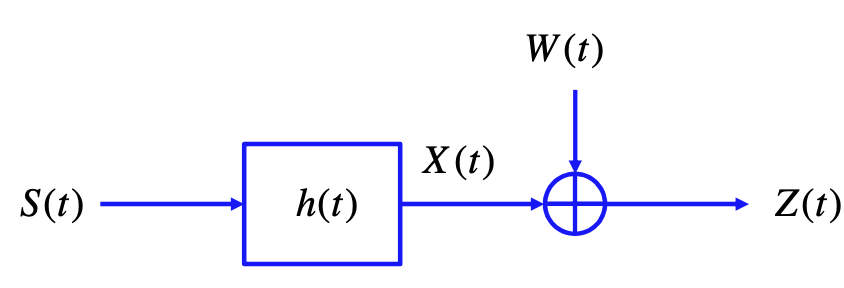
\includegraphics[width=0.65\linewidth]{Image/pdf 8/5.Deconvolution.png}
        \label{fig:placeholder}
    \end{figure}
    \item \textbf{Problem}: retrive (estimate) \(S(t)\), given the observation \(Z(t)\) in the interval \([0,T)\).
    \item \textbf{Assumption}: the random signal \(S(t)\) is bandlimited with bandwidth \(B_s\) (or essential bandwidth at level \(\alpha\ll1\) equal to \(B_s\)).
\begin{figure}[H]
    \centering
    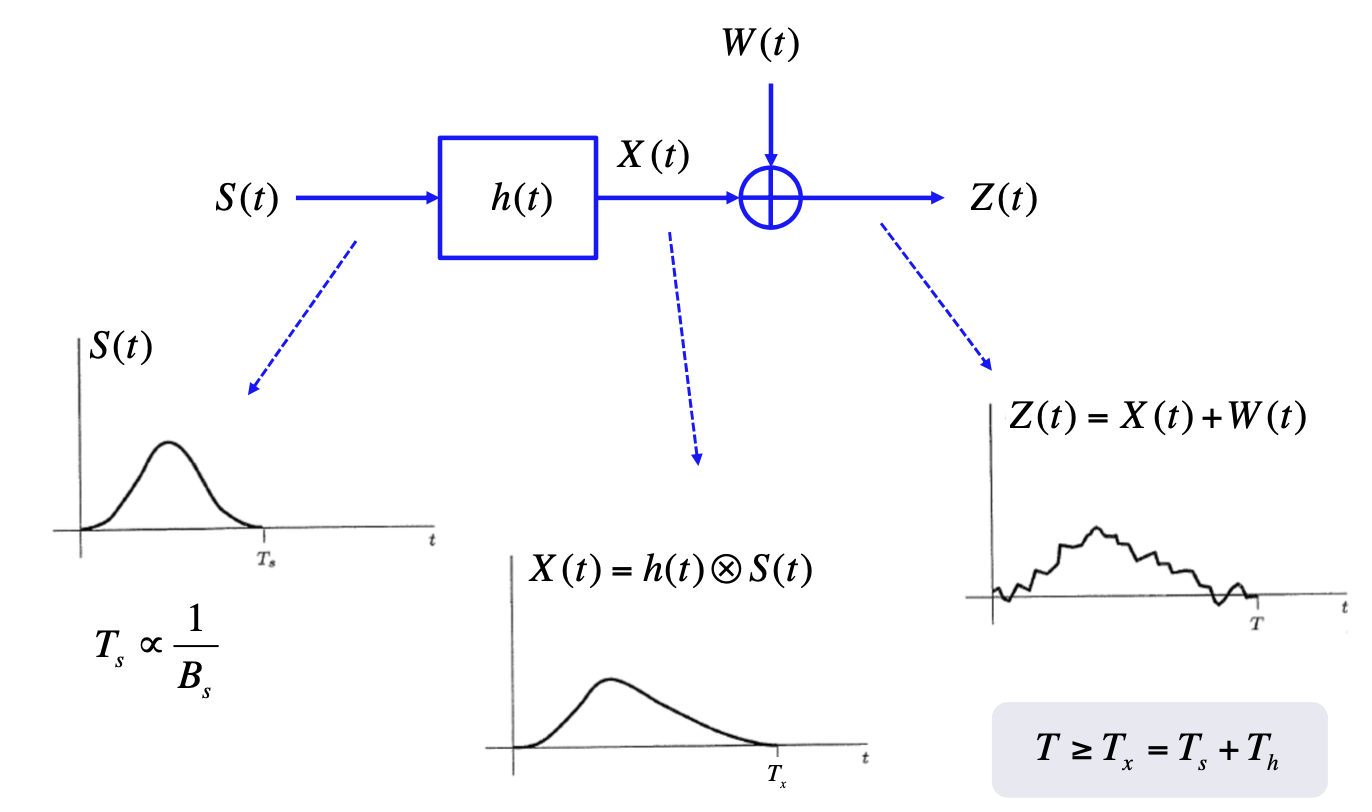
\includegraphics[width=0.65\linewidth]{Image/pdf 8/6.Deconv_2.png}
    \label{fig:placeholder}
\end{figure}
\item To represent the received signal \(Z(t)\) in discrete format, first we filter the received signal with an \textit{anti-aliasing} filter \(h_{LP}(t)\), low-pass with bandwidth \(B\geq B_s\), such that \(2BT\gg1\), and then we sample the received signal in the interval \([0,T)\) with sampling frequency \(F_c=2B\), i.e. sampling interval \(T_c=1/2B\) collecting, \(N=2BT\) samples.
$$
Z(t)\otimes h_{LP}(t) = [X(t)+W(t)]\otimes h_{LP}(t) = X(t)\otimes h_{LP}(t) + W(t)\otimes h_{LP}(t)
$$
\item As concerning the useful signal:
$$
X(t)\otimes h_{LP}(t) = S(t)\otimes h(t)\otimes h_{LP}(t) \approx S(t)\otimes h(t) = X(t)
$$
\item As concerning the noise component:
$$
W_{B}(t) = W(t)\otimes h_{LP}(t) \implies S_{W_{B}}(f) = S_{W}(f)|H_{LP}(f)|^2 = \frac{N_0}{2}rect\left(\frac{f}{2B}\right)
$$
\item We sample at intervals \(T_c=1/2B\) and we collect \(N=2BT\) samples:
\begin{align*}
&\ Z_k \triangleq \frac{1}{\sqrt{2B}}\left[Z(t)\otimes h_{LP}(t)\right]_{t=\frac{k}{2B}} = \frac{1}{\sqrt{2B}}X\left(\frac{k}{2B}\right) + \frac{1}{\sqrt{2B}}W_{B}\left(\frac{k}{2B}\right) \\[8pt]
& \left\{ W_{k} \triangleq \frac{1}{\sqrt{2B}}W_{B}\left(\frac{k}{2B}\right) \right\}_{k=0}^{N-1} \quad \text{uncorrelated, Gaussian distributed, zero mean} \\[8pt]
&\text{and variance } \sigma_{W}^2 = \frac{N_0}{2} \implies W_k \in \mathcal{N}\left(0, \frac{N_0}{2}\right), \text{ IID} \\[8pt]
& X_k \triangleq \frac{1}{\sqrt{2B}}X\left(\frac{k}{2B}\right) = \frac{1}{\sqrt{2B}}\left[\int_{0}^{T} S(\tau)h(t-\tau)d\tau\right]_{t=\frac{k}{2B}}, \quad k=0, 1, 2, \dots, N-1\\[8pt]
&X_k \triangleq \frac{1}{\sqrt{2B}}X\left(\frac{k}{2B}\right) = \frac{1}{\sqrt{2B}}\int_{0}^{T} S(\tau)h\left(\frac{k}{2B}-\tau\right)d\tau
\end{align*}
\item Approximating the integral with the rule of rectangles:
$$
X_k \approx \frac{1}{\sqrt{2B}}\sum_{i=0}^{N_p-1} S(i\Delta T)h\left(\frac{k}{2B}-i\Delta T\right)\cdot \Delta T, \quad \text{where } N_p = \frac{T}{\Delta T}
$$
\item The approximation is accurate if \(N_p\gg1\). Let us assume \(\Delta T=1/2B\), so we get \(N_p=N=2BT\):
$$
X_k \approx \sum_{i=0}^{N-1}\frac{1}{\sqrt{2B}}S\left(\frac{i}{2B}\right)h\left(\frac{k}{2B}-\frac{i}{2B}\right)\cdot \frac{1}{2B}, \quad \text{where } N = 2BT
$$
\item Now, define: 
$$
S_k \triangleq \frac{1}{\sqrt{2B}}S\left(\frac{k}{2B}\right), \quad h_k \triangleq \frac{1}{2B}h\left(\frac{k}{2B}\right)
$$
\item We get the \textbf{Equivalent discrete-time system}:
$$
X_k \approx \sum_{i=0}^{N-1}S_i h_{k-i} = S_k \otimes h_k \implies Z_k = X_k + W_k = S_k \otimes h_k + W_k
$$
\begin{figure}[H]
    \centering
    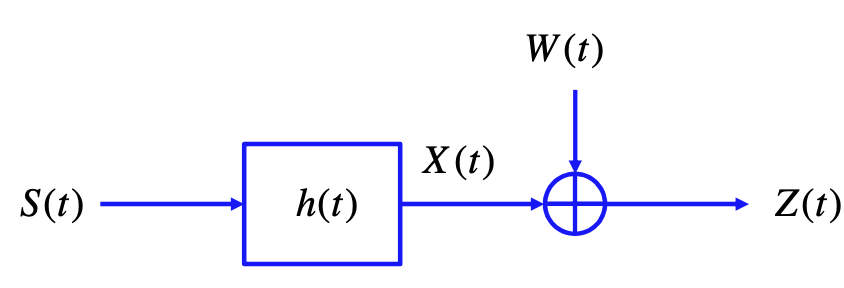
\includegraphics[width=0.65\linewidth]{Image/pdf 8/5.Deconvolution.png}
    \label{fig:placeholder}
\end{figure}
\item If \(S(t)\) has duration \(T_s<T\), then \(S_k\) has duration \(N_s=T_s/T_c=2BT_s<N\).
\item If \(h(t)\) has duration \(T_h<T\), then \(h_k\) has duration \(N_h=T_h/T_c=2BT_h<N\).
\item The convolution between \(S_k\) and \(h_k\) has duration \(N_s+N_h-1\) so \(N\geq N_s+N_h-1\).
\item Let us assume that \(T=T_s+T_h\), so that \(N=N_s+N_h-1\)
\item Recalling that \(S_i=0\) if \(i<0\) or \(i\geq N_s\), the observed data samples are given by:
\begin{align*}
&Z_k = \sum_{i=0}^{N_s-1} S_i h_{k-i} + W_k, \quad k=0, 1, 2, \dots, N-1 \\[8pt]
&= S_0 h_k + S_1 h_{k-1} + \dots + S_{N_s-1} h_{k-(N_s-1)} + W_k \\[15pt]
&\begin{cases}
k=0: & Z_0 = S_0 h_0 + S_1 h_{-1} + \dots + S_{N_s-1} h_{-(N_s-1)} + W_0 \\
k=1: & Z_1 = S_0 h_1 + S_1 h_0 + \dots + S_{N_s-1} h_{1-(N_s-1)} + W_1 \\
\vdots \\
k=N-1: & Z_{N-1} = S_0 h_{N-1} + S_1 h_{N-2} + \dots + S_{N_s-1} h_{N-1-(N_s-1)} + W_{N-1}
\end{cases}
\end{align*}
\item In vector format (keeping in mind that \(h_k\) is a causal filter with memory \(N_h\),i.e. \(h_k=0\) for \(k<0\) and \(k\geq N_h\)):

$$
\underbrace{\left[
\begin{array}{c}
Z_0 \\
Z_1 \\
Z_2 \\
\vdots \\
Z_{N-1}
\end{array}
\right]}_{\mathbf{Z}}
=
\underbrace{\left[
\begin{array}{cccccc}
h_0 & 0 & \cdots & \cdots & 0 & 0 \\
h_1 & h_0 & 0 & \cdots & \cdots & 0 \\
h_2 & h_1 & h_0 & 0 & \cdots & 0 \\
\vdots & h_2 & h_1 & \ddots & & \vdots \\
h_{N_h-1} & \vdots & \ddots & \ddots & h_0 & 0 \\
0 & h_{N_h-1} & & \ddots & h_1 & h_0 \\
\vdots & 0 & h_{N_h-1} & \cdots & h_2 & h_1 \\
\vdots & \vdots & 0 & \ddots & \vdots & h_2 \\
0 & 0 & \cdots & 0 & 0 & h_{N_h-1}
\end{array}
\right]}_{\underset{N \times N_s}{\mathbf{H}}}
\underbrace{\left[
\begin{array}{c}
S_0 \\
S_1 \\
\vdots \\
S_{N_s-1}
\end{array}
\right]}_{\mathbf{S}}
+
\underbrace{\left[
\begin{array}{c}
W_0 \\
W_1 \\
\vdots \\
W_{N-1}
\end{array}
\right]}_{\mathbf{W}}
$$
$$
\mathbf{Z} = \mathbf{H} \cdot \mathbf{S} + \mathbf{W}, \quad \text{where } N = N_s + N_h - 1 > N_s
$$
\item Hence, the problem is exaclty in the form of a \textbf{linear signal model} that we have already investigated, both the case of deterministic signal (\textbf{S} is a deterministic unknown vector) and the case of random signal (\textbf{S} ia random vector).
\item Assume now that \(S(t)\) is a WSS random process, not necessarily Gaussian, with zero mean function and known autocorrelation function (ACF) \(R_s(\tau)\).
\item In this case, we get the \textbf{Bayesian linear model:} \(\mathbf{Z=HS+W}\):
\begin{align*}
&\mathbf{W}\in\mathcal{N}\left(\mathbf{0}, \frac{N_0}{2}\mathbf{I}\right), \quad \mathbf{H} \text{ known}, \quad \boldsymbol{\eta}_{\mathbf{S}} = E\{\mathbf{S}\} = \mathbf{0}, \quad \mathbf{C}_{\mathbf{S}} = E\{\mathbf{S}\mathbf{S}^{T}\} \\[8pt]
&\left[\mathbf{C}_{\mathbf{S}}\right]_{i+1, k+1} = E\left\{S_i S_k\right\} = E\left\{\frac{1}{\sqrt{2B}}S\left(\frac{i}{2B}\right)\frac{1}{\sqrt{2B}}S\left(\frac{k}{2B}\right)\right\} = \frac{1}{2B}R_S\left(\frac{k-i}{2B}\right) \\[8pt]
&i, k = 0, 1, 2, \dots, N_s-1
\end{align*}
\item The LMMSE estimator of \textbf{S} is given \textbf{Z} is known:
$$
\begin{cases}
\hat{\mathbf{S}}_{\text{LMMSE}} = \mathbf{C}_{\mathbf{S}}\mathbf{H}^{T}\left(\mathbf{H}\mathbf{C}_{\mathbf{S}}\mathbf{H}^{T} + \frac{N_0}{2}\mathbf{I}\right)^{-1} \mathbf{Z} \\[8pt]
\mathbf{C}_{\varepsilon} = \left(\mathbf{C}_{\mathbf{S}}^{-1} + \frac{2}{N_0}\mathbf{H}^{T}\mathbf{H}\right)^{-1} \to \text{MSE}\{\hat{S}_{i,\text{LMMSE}}\} = [\mathbf{C}_{\varepsilon}]_{i,i}
\end{cases}
$$
\item If \(S(t)\) is a Gaussian process, then \textbf{S} is a Gaussian vector and the LMMSE estimator is also the MMSE (and MAP) estimator.

(ESEMPIO NUMERICO PDF 8 96-100)
\end{itemize}
\subsection{Channel Identification}
\begin{itemize}
    \item \textbf{Channel identification}: \(\{S_i\}\) is known (\(S_i=0\) for \(i<0\) or \(i\geq N_s\)) and the problem is to estimate \(\{h_i\}\).
    \item Recalling that the filter is causal and with finite memory, i.e. \(h_i=0\) for \(i<0\) or \(i\geq N_h\), the observed data sample are given by:
    \begin{align*}
Z_k &= \sum_{i=0}^{N_s-1} S_i h_{k-i} + W_k = \sum_{i=0}^{N_h-1} h_i S_{k-i} + W_k, \quad k=0, 1, 2, \dots, N-1 \\[8pt]
&= h_0 S_k + h_1 S_{k-1} + \dots + h_{N_h-1} S_{k-(N_h-1)} + W_k \\[15pt]
&\begin{cases}
k=0: & Z_0 = h_0 S_0 + h_1 S_{-1} + \dots + h_{N_h-1} S_{-(N_h-1)} + W_0 \\
k=1: & Z_1 = h_0 S_1 + h_1 S_0 + \dots + h_{N_h-1} S_{1-(N_h-1)} + W_1 \\
\vdots \\
k=N-1: & Z_{N-1} = h_0 S_{N-1} + h_1 S_{N-2} + \dots + h_{N_h-1} S_{N-1-(N_h-1)} + W_{N-1}
\end{cases}
\end{align*}


$$
\underbrace{
\left[
\begin{array}{c}
Z_0 \\
Z_1 \\
\vdots \\
Z_{N-1}
\end{array}
\right]
}_{\mathbf{Z}}
=
\underbrace{
\left[
\begin{array}{ccccc}
S_0 & 0 & \cdots & \cdots & 0 \\
S_1 & S_0 & 0 & \cdots & 0 \\
S_2 & S_1 & S_0 & 0 & \vdots \\
\vdots & \ddots & \ddots & \ddots & 0 \\
S_{N_s-1} & \vdots & \ddots & S_1 & S_0 \\
0 & S_{N_s-1} & & \ddots & S_1 \\
\vdots & 0 & S_{N_s-1} & \cdots & S_2 \\
\vdots & \vdots & 0 & \ddots & \vdots \\
0 & 0 & \cdots & 0 & S_{N_s-1}
\end{array}
\right]
}_{\mathbf{S}_{N \times N_h}}
\underbrace{
\left[
\begin{array}{c}
h_0 \\
h_1 \\
\vdots \\
h_{N_h-1}
\end{array}
\right]
}_{\mathbf{h}}
+
\underbrace{
\left[
\begin{array}{c}
W_0 \\
W_1 \\
\vdots \\
W_{N-1}
\end{array}
\right]
}_{\mathbf{W}}
$$
$$
\mathbf{Z} = \mathbf{S} \cdot \mathbf{h} + \mathbf{W}, \quad \text{where } N = N_s + N_h - 1 > N_h
$$
\item The \textbf{LMMSE estimator} of \textbf{h} given \textbf{Z} is given by:

$$
\hat{\mathbf{h}}_{\text{LMMSE}} = \mathbf{C}_{\mathbf{h}}\mathbf{S}^{T}\left(\mathbf{S}\mathbf{C}_{\mathbf{h}}\mathbf{S}^{T} + \frac{N_0}{2}\mathbf{I}\right)^{-1} \mathbf{Z}
$$

\item If the channel is \underline{deterministic}(so we do not have \(\mathbf{C}_h\)), we can derive the \textbf{linear LS estimator} of \textbf{h}:

$$
\hat{\mathbf{h}}_{\text{LS}} = \mathbf{S}^{\#}\mathbf{Z} = (\mathbf{S}^{T}\mathbf{S})^{-1}\mathbf{S}^{T}\mathbf{Z}
$$
(SEQUENTIAL RECURSIVE NOT IN THE PROGRAMME)
\end{itemize}




\clearpage









